\documentclass[10pt, a4paper]{article}

\usepackage[utf8]{inputenc}
\usepackage[spanish]{babel} 
\usepackage[margin = 1in]{geometry} 
\usepackage{caratula}
\usepackage{algorithmicx}
\usepackage{algpseudocode}
\usepackage[Algoritmo]{algorithm}
\usepackage[fleqn]{amsmath}
\usepackage{amssymb}
\usepackage{color}
\usepackage{url}
\usepackage[colorlinks = true, linkcolor = blue]{hyperref}
\usepackage{comment}
\usepackage{hyperref}

\usepackage{listings}
\usepackage{listingsutf8}
\usepackage{color}

\usepackage{wrapfig}
\usepackage{nccmath}
\usepackage{caption}
\usepackage{subcaption}

\usepackage{mathtools}

\definecolor{codegreen}{rgb}{0,0.6,0}
\definecolor{codegray}{rgb}{0.5,0.5,0.5}
\definecolor{codepurple}{rgb}{0.58,0,0.82}
\definecolor{backcolour}{rgb}{0.95,0.95,0.92}

\lstset{inputencoding=utf8/latin1,
  language=C++,
  basicstyle=\ttfamily,
  keywordstyle=\bfseries\color{blue},
  stringstyle=\color{red}\ttfamily,
  commentstyle=\color{mygreen}\ttfamily,
  morecomment=[l][\color{magenta}]{\#},
  % numbers=left,
  numberstyle=\color{gray},
  backgroundcolor=\color{backcolour},   
  keywordstyle=\color{magenta},
  breakatwhitespace=false,
  breaklines=true,
  captionpos=b,
  keepspaces=true,
  numbersep=5pt,
  showspaces=false,
  showstringspaces=false,
  showtabs=false,
  tabsize=3,
  inputencoding=utf8/latin1
}

% Para que tenga acentos el environment lstlisting
\lstset{
     literate=%
         {á}{{\'a}}1
         {í}{{\'i}}1
         {é}{{\'e}}1
         {ý}{{\'y}}1
         {ú}{{\'u}}1
         {ó}{{\'o}}1
         {ě}{{\v{e}}}1
         {š}{{\v{s}}}1
         {č}{{\v{c}}}1
         {ř}{{\v{r}}}1
         {ž}{{\v{z}}}1
         {ď}{{\v{d}}}1
         {ť}{{\v{t}}}1
         {ň}{{\v{n}}}1                
         {ů}{{\r{u}}}1
         {Á}{{\'A}}1
         {Í}{{\'I}}1
         {É}{{\'E}}1
         {Ý}{{\'Y}}1
         {Ú}{{\'U}}1
         {Ó}{{\'O}}1
         {Ě}{{\v{E}}}1
         {Š}{{\v{S}}}1
         {Č}{{\v{C}}}1
         {Ř}{{\v{R}}}1
         {Ž}{{\v{Z}}}1
         {Ď}{{\v{D}}}1
         {Ť}{{\v{T}}}1
         {Ň}{{\v{N}}}1                
         {Ů}{{\r{U}}}1    
}

\hypersetup{urlcolor=blue}

\makeatletter
\newenvironment{breakablealgorithm}
  {% \begin{breakablealgorithm}
   \begin{center}
     \refstepcounter{algorithm}% New algorithm
     \hrule height.8pt depth0pt \kern2pt% \@fs@pre for \@fs@ruled
     \renewcommand{\caption}[2][\relax]{% Make a new \caption
       {\raggedright\textbf{\ALG@name~\thealgorithm} ##2\par}%
       \ifx\relax##1\relax % #1 is \relax
         \addcontentsline{loa}{algorithm}{\protect\numberline{\thealgorithm}##2}%
       \else % #1 is not \relax
         \addcontentsline{loa}{algorithm}{\protect\numberline{\thealgorithm}##1}%
       \fi
       \kern2pt\hrule\kern2pt
     }
  }{% \end{breakablealgorithm}
     \kern2pt\hrule\relax% \@fs@post for \@fs@ruled
   \end{center}
  }
\makeatother

\newcommand{\bigo}[1]{\ensuremath{\mathcal{O}(#1)}}

\begin{document}

\titulo{Trabajo práctico}

\subtitulo{\textit{Extended Formulations and Branch-and-Cut Algorithms for the Black-and-White Traveling Salesman Problem}}

\materia{Seminario Avanzado de Programación Lineal Entera}

\integrante{Bogdanich Espina, Vera}{601/14}{verabogdanichespina@gmail.com}
\integrante{Puterman Colomer, Lucas}{COMPLETAR}{lucasputerman@gmail.com}

\maketitle

\tableofcontents

\newpage

\section{Introducción}

En este trabajo$^{\cite{main}}$ estudian una variante del problema del viajante de comercio: \textit{el problema del viajante de comercio blanco y negro}, o BWTSP por \textit{black-and-white travelling salesman problem}.

El BWTSP está definido sobre un grafo no dirigido que tiene su conjunto de vértices divido en dos, los blancos W y los negros B. Además, cada arista tiene una distancia d y un costo c asociado. El objetivo es encontrar el camino de longitud mínima que recorre todos los vértices, y en el que el trayecto entre dos nodos negros consecutivos contiene al menos Q nodos blancos y tiene una distancia de L como máximo. En la figura \ref{fig:ejemplo_0} se puede ver una instancia del problema junto con su solución.

\begin{figure}[H]
    \centering
    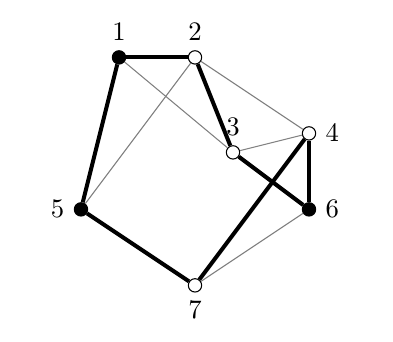
\includegraphics[width=0.4\textwidth]{ejemplo_0.png}
    \caption{Una instancia con B = \textbraceleft 1, 5, 6\textbraceright, W = \textbraceleft 2, 3, 4, 7\textbraceright, y una solución factible indicada por las aristas gruesas para Q = 2 y L = 3. La solución es óptima, por ejemplo, cuando el costo y la distancia de cada arista es 1 para todas las contenidas en la solución, y 2 para el resto.}
    \label{fig:ejemplo_0}
\end{figure}

Entre las aplicaciones de este problema están las operaciones aéreas de trayectos cortos. En este caso los vértices negros pueden representar estaciones de mantenimiento que los aviones tienen que visitar después de Q + 1 tramos como máximo, o después de haber recorrido una distancia máxima de L.

\section{Modelos}

(Sección para explicar qué es un modelo de PLE y el genérico que está en la introducción del paper)

\begin{align} 
	\min & \sum_{e \in E} c_{e} x_{e} & \label{eq:1} \\
	\text {tal que} & \quad x(\delta(i))=2 & \forall i \in V \label{eq:2} \\
	& x(E(S)) \geq 2 & \forall S \subseteq V \backslash\{1\},\ S \neq \emptyset \label{eq:3} \\
	& \left\{e \in E : x_{e}=1\right\} & \text { satisface la restricción de salto para el camino después de cada } k \in B \label{eq:4} \\
	& \left\{e \in E : x_{e}=1\right\} & \text { satisface la restricción de distancia para el camino después de cada } k \in B \label{eq:5} \\
	& \mathbf{x} \in\{0,1\}^{|E|} & \label{eq:6}
\end{align}

\section{Modelo de porción del camino}

\begin{align} 
	& x^{k}\left(\delta^{+}(k)\right)=1 & \forall k \in B \label{eq:7} \\
	& \sum_{j \in B \backslash\{k\}} x^{j}\left(\delta^{-}(k)\right)=1 & \forall k \in B \label{eq:8} \\
	& x^{k}\left(\delta^{-}(i)\right)=x^{k}\left(\delta^{+}(i)\right) & \forall k \in B,\ \forall i \in W \label{eq:9} \\
	& \sum_{k \in B} x_{i j}^{k}+x_{j i}^{k}=x_{e} & \forall e=\{i, j\} \in E \label{eq:10}
\end{align}

\begin{align} 
	& \sum_{e=\{i, j\} \in E}\left(x_{i j}^{k}+x_{j i}^{k}\right) \leq Q+1 & \forall k \in B \label{eq:11} \\
	& \sum_{e=\{i, j\} \in E} d_{e}\left(x_{i j}^{k}+x_{j i}^{k}\right) \leq L & \forall k \in B \label{eq:12}
\end{align}

\begin{align}
	& x^{k}\left(\delta^{-}(j)\right)+x^{j}\left(\delta^{-}(k)\right) \leq 1 & \forall k \neq j \in B \label{eq:13}
\end{align}

\section{Formulaciones dependientes de la posición}

\subsection{Formulación pura}

\begin{align}
	& X^{1}\left(\delta^{+}(k)\right)=1 & \forall k \in B \label{eq:14} \\
	& \sum_{p=1}^{Q+1} X^{p}\left(\delta^{-}(k)\right)=1 & \forall k \in B \label{eq:15} \\
	& X^{p}\left(\delta^{-}(i)\right)=X^{p+1}\left(\delta^{+}(i)\right) & \forall i \in W,\ \forall p \in\{1,2, \ldots, Q\} \label{eq:16} \\
	& \sum_{p=1}^{Q+1}\left(X_{i j}^{p}+X_{j i}^{p}\right)=x_{e} & \forall e=\{i, j\} \in E \label{eq:17}
\end{align}

\begin{align}
	& \sum_{e \in P} x_{e} \leq|P|-1 & \forall P \in \mathcal{P}_{\mathrm{inf}} \label{eq:18}
\end{align}

\begin{align}
	& X_{i j}^{p} \leq \sum_{h \neq i} X_{j h}^{p+1} & \forall p \in\{1,2, \ldots, Q\},\ \forall e=\{i, j\} \in E, j \in W \label{eq:19} \\
	& X_{i j}^{p} \leq \sum_{h \neq i} X_{j h}^{1} & \forall p \in\{1,2, \ldots, Q+1\},\ \forall e=\{i, j\} \in E, j \in B \label{eq:20}
\end{align}

\begin{align}
	& X\left(\delta^{-}(S)\right) \geq 1 & \forall S \subseteq V_{\mathrm{Q}} \backslash\left\{j_{0} : j \in B\right\}, \exists i \in W |\left\{i_{p}, p \in\{1,2, \ldots, Q\}\right\} \subseteq S \label{eq:21}
\end{align}

\subsection{Formulación de una porción del camino}

(Modelos traducidos así nomás. Hay que mejorar seguro este)

\begin{align}
	& Y^{k, 1}\left(\delta^{+}(k)\right)=1 & \forall k \in B \label{eq:22} \\
	& \sum_{j \in B \backslash\{k\}} \sum_{p=1}^{Q+1} Y^{j, p}\left(\delta^{-}(k)\right)=1 & \forall k \in B \label{eq:23} \\
	& Y^{k, p}\left(\delta^{-}(i)\right)=Y^{k, p+1}\left(\delta^{+}(i)\right) & \forall k \in B, \forall i \in W, \forall p \in\{1, \ldots, Q\} \label{eq:24} \\
	& \sum_{k \in B} \sum_{p=1}^{Q+1}\left(Y_{i j}^{k, p}+Y_{j i}^{k, p}\right)=x_{e} & \forall e=\{i, j\} \in E \label{eq:25}
\end{align}

\begin{align}
	& \sum_{p=1}^{Q+1} \sum_{e=\{i, j\} \in E} d_{e}\left(Y_{i j}^{k, p}+Y_{j i}^{k, p}\right) \leq L & \forall k \in B \label{eq:26}
\end{align}

\begin{align}
	& Y_{i j}^{k, p} \leq \sum_{h \neq i} Y_{j h}^{k, p+1} & \forall k \in B,\ \forall p \in\{1,2, \ldots, Q\}, \forall e=\{i, j\} \in E, j \in W \label{eq:27} \\
	& Y_{i j}^{k, p} \leq \sum_{h \neq i} Y_{j h}^{j, 1} & \forall k \in B,\ \forall p \in\{1,2, \ldots, Q+1\}, \forall e=\{i, j\} \in E, j \in B \backslash\{k\} \label{eq:28}
\end{align}

\begin{align}
	& Y\left(\delta^{-}(S)\right) \geq 1 & \forall S \subseteq V_{\mathrm{QB}} \backslash\{j_{0}^{j} : j \in B\},\ \exists i \in W |\left\{i_{p}^{k}, k \in B, p \in\{1,2, \ldots, Q\}\right\} \subseteq S \label{eq:29}
\end{align}

\subsection{Modelo 2-dimensional}

\begin{align}
	& Z^{1,1}\left(\delta^{+}(1)\right)=1 \label{eq:30} \\
	& \sum_{j \in B \backslash\{1\}} Z^{m, 1}\left(\delta^{+}(j)\right)=1 & \forall m \in\{2,3, \ldots,|B|\} \label{eq:31} \\
	& \sum_{i \in V \backslash\{1\}} \sum_{p=1}^{Q+1} \sum_{p=1} \sum_{i 1}^{|B|, p}=1 \label{eq:32} \\
	& \sum_{i \in V} \sum_{p=1}^{Q+1} \sum_{p=1} Z_{i k}^{m, p}=1 & \forall m \in\{2,3, \ldots,|B|\},\ \forall k \in B \backslash\{1\} \label{eq:33} \\
	& Z^{m, p}\left(\delta^{-}(i)\right)=Z^{m, p+1}\left(\delta^{+}(i)\right) & \forall m \in\{1,2, \ldots,|B|\}, \forall p \in\{1,2, \ldots, Q\},\ \forall i \in W \label{eq:34} \\
	& \sum_{m=1}^{|B|} \sum_{p=1}^{Q+1}\left(Z_{i j}^{m, p}+Z_{j i}^{m, p}\right)=x_{e} & \forall e=\{i, j\} \in E \label{eq:35}
\end{align}

\begin{align}
	& \sum_{p=0}^{Q} \sum_{e=\{i, j\} \in E} d_{e}\left(Z_{i j}^{m, p}+Z_{j i}^{m, p}\right) \leq L \quad \forall m \in\{1,2, \ldots,|B|\} \label{eq:36}
\end{align}

\begin{align}
	& Z_{i j}^{m, p} \leq \sum_{h \neq i} Z_{j h}^{m, p+1} & \forall m \in\{1,2, \ldots,|B|\},\ \forall p \in\{1,2, \ldots, Q\},\ \forall e=\{i, j\} \in E, j \in W \label{eq:37} \\
	& Z_{i j}^{m, p} \leq \sum_{h \neq i} Z_{j h}^{m+1,1} & \forall m \in\{1,2, \ldots,|B|-1\},\ \forall p \in\{1,2, \ldots, Q+1\},\ \forall e=\{i, j\} \in E, j \in B \backslash\{1\} \label{eq:38} \\
	& Z_{i 1}^{|B|, p} \leq \sum_{h \neq i} Z_{1 h}^{1,1} & \forall p \in\{1,2, \ldots, Q+1\},\ \forall e=\{i, 1\} \in E \label{eq:39}
\end{align}

\begin{multline}
	 Z(\delta^{-}(S)) \geq 1 \quad \quad \forall S \subseteq V_{\mathrm{QI}} \backslash\{i_{0}^{m} | i \in B, m \in\{1,2, \ldots,|B|\}, \\
	 \exists i \in W : \{i_{p}^{m} | p \in \{1,2, \ldots, Q\}, m \in \{1,2, \ldots,|B|\}\} \subseteq S \label{eq:40}
\end{multline}

\section{Modelos alternativos dependientes del tiempo}

\section{Comparaciones teóricas}

\section{Algoritmos de ramificación y corte}

(Explicar bien todo el concepto, que podría introducirse también más arriba para entender para qué son los modelos)

\subsection{Pre-procesamiento}

\subsection{Algoritmo de plano de corte}

\subsection{Heurísticas}

\section{Resultados empíricos}

(Por ahí habría que mejorar este título)

\subsection{Instancias}

\subsection{Relajaciones}

\subsection{Análisis de los resultados}

\pagebreak

\begin{thebibliography}{9}

\bibitem{main}
L. Gouveia, M. Leitner y M. Ruthmair, “Extended formulations and branch-and-cut algorithms for the Black-and-White Traveling Salesman Problem". European Journal of Operational Research, 262-3, 908-928. 2017.

\end{thebibliography}

\end{document}